\documentclass[11pt]{scrartcl}
\usepackage[utf8]{inputenc}
\usepackage[sexy]{evanchen} 
\usepackage{graphicx}
\graphicspath{{8 Outsource K Math/Gambar/}}

\title{Segitiga}
\author{Azzam and Akeyla}
\date{Maret 2023}

\begin{document}

\maketitle

\section{Properti Segitiga}
\subsection{Ketaksamaan Segitiga}
Jika $a,b,c$ adalah panjang dari ketiga titik segitiga, maka 
\begin{align*}
    a+b>c\\
    b+c>a\\
    c+a>b\\
\end{align*}
Dengan kata lain, panjang sisi terpanjang segitiga pasti lebih pendek daripada jumlah kedua sisinya yang lain.

\subsection{Luas Segitiga}
Luas segitiga dapat dicari dengan berbagai cara. Tiga cara yang umum digunakan adalah
\begin{enumerate}
    \item Apabila diketahui panjang salah satu sisi segitiga dan panjang garis tinggi ke sisi tersebut, maka dapat digunakan rumus \[L= \dfrac{1}{2}at\] dengan $a$ adalah panjang sisi segitiga dan $t$ adalah panjang garis tinggi yang sesuai.
    \item Apabila diketahui panjang dua buah sisi dan besar sudut yang diapit kedua sisi tersebut, dapat digunakan rumus \[L = \dfrac{1}{2} ab \sin{\gamma}\] dengan $a$ dan $b$ adalah dua buah sisi yang dimaksud dan $\gamma$ adalah besar sudut yang diapit kedua sisi tersebut.
    \item Apabila diketahui panjang ketiga sisi segitiga tersebut, dapat digunakan dalil Heron: \[L=\sqrt{s(s-a)(s-b)(s-c)}\] dengan $a,b,c$ adalah panjang ketiga sisi segitiga dan $s=\dfrac{(a+b+c)}{2}$
\end{enumerate}
Selain itu, apabila ada tiga titik $A, B, C$ yang segaris dan titik $X$ yang tidak segaris dengan ketiganya, maka perbandingan luas segitiga $XAB, XBC,$ dan $XCA$ akan sama dengan perbandingan panjang sisi $AB, BC, CA$.
\subsection{Dalil Stewart}
Dalil Stewart digunakan untuk mencari panjang sebuah segmen garis yang menghubungkan sebuah titik sudut segitiga dan sisi yang ada di hadapannya di titik sembarang. \\
\begin{figure}[h]
    \centering
    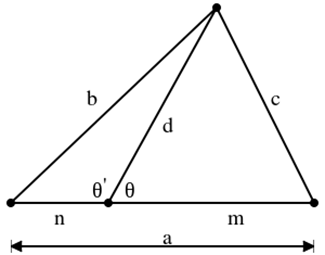
\includegraphics{Stewart.png}
    \caption{Dalil Stewart}
    \label{fig:my_label}
\end{figure}

Pada gambar di atas, berlaku hubungan
\[b^2 m+c^2 n=a(d^2+mn)\]

\subsection{Dalil Cosinus dan Dalil Sinus}
Asumsikan kita memiliki sebuah segitiga $ABC$ dengan panjang sisi $AB = c, BC = a, CA = b$ dan besar sudut $\angle{ABC} = \beta, \angle{CAB} = \alpha, \angle{BCA} = \gamma$.
\begin{enumerate}
    \item \textbf{Dalil Cosinus}\\
    \[a^2 = b^2 + c^2 - 2bc\cos{\alpha}\]
    \[b^2 = c^2 + a^2 - 2ca\cos{\beta}\]
    \[c^2 = a^2 + b^2 - 2ab\cos{\gamma}\]
    \item \textbf{Dalil Sinus}\\
    \[\dfrac{a}{\sin{\alpha}} = \dfrac{b}{\sin{\beta}} = \dfrac{c}{\sin{\gamma}}\]
\end{enumerate}

\section{Beberapa Identitas Trigonometri Sederhana}
\begin{enumerate}
    \item $\sin^2 x + \cos^2 x = 1$
    \item $\sin(x \pm y) = \sin x \cos y \pm \cos x \sin y$
    \item $\cos(x \pm y) = \cos x \cos y \mp \sin x \sin y$
    \item $\sin(180^{\circ} - x) = \sin x$
    \item $\cos(180^{\circ} - x) = -\cos x$
    \item $\sin 2x = 2\sin x \cos x$
    \item $\cos 2x = \cos^2 x - \sin^2 x = 1 - 2\sin^2 x = 2\cos^2 x - 1$
    \item $\sin 3x = 3\sin x - 4\sin^3 x$
    \item $\cos 3x = 4\cos^3 x - 3\cos x$
\end{enumerate}

\section{Latihan Komprehensif}
\begin{problem}
    % Ketaksamaan segitiga
    Sebuah segitiga memiliki panjang $20, 24,$ dan $n$ dengan $n$ merupakan sebuah bilangan asli. Semua nilai $n$ yang mungkin adalah ...
\end{problem}

\begin{problem}
% Stewart
    Diberikan sebuah segitiga $ABC$ dengan $AB = c, BC = a,$ dan $CA = b$. Titik $D$ adalah titik tengah sisi $BC$. Nyatakan panjang $AD$ dalam $a, b,$ dan $c$.
\end{problem}

\begin{problem}
    Sebuah segitiga memiliki keliling $8$ dan seluruh panjang sisinya merupakan bilangan asli. Luas dari segitiga tersebut adalah ...
\end{problem}

\begin{problem}
Diberikan sebuah persegi $ABC$ dengan panjang sisi $10$. Titik $E$ terletak di diagonal $DB$ sedemikian hingga $BE = 2DE$. Titik $F$ terletak di segmen garis $AE$ sedemikian hingga $AF = 2FE$. Luas segitiga $BFE$ adalah ...
\begin{figure}[h]
    \centering
    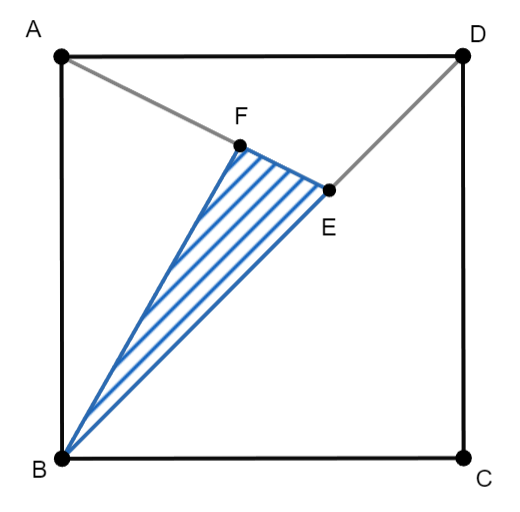
\includegraphics[width=0.3\linewidth]{perbandinganluassegitiga.png}    
\end{figure}
\end{problem}

\begin{problem}
    % Dalil sinus/kosinus 
    Diberikan segitiga $ABC$ dengan $\angle A = 2\angle B$. Jika $AB = 3$ dan $AC = 2$. Tentukan panjang $BC$.
\end{problem}

\begin{problem}
    % https://artofproblemsolving.com/community/c5h1784834p11779482
    (AMC 2019 12B) 
    Diberikan sebuah segitiga siku-siku sama kaki $ABC$ yang siku-siku di $B$ dan panjang sisi kakinya adalah $1$. Konstruksikan sebuah segitiga siku-siku $ACD$ yang siku-siku di $C$ dan $D$ terletak di sisi yang berbeda dari $B$ terhadap $AC$ sedemikian hingga segitiga $ABC$ dan $ADC$ memiliki keliling yang sama. Nilai dari $\sin{2\angle{BAD}}$ adalah ...
    \begin{figure}[h]
        \centering
        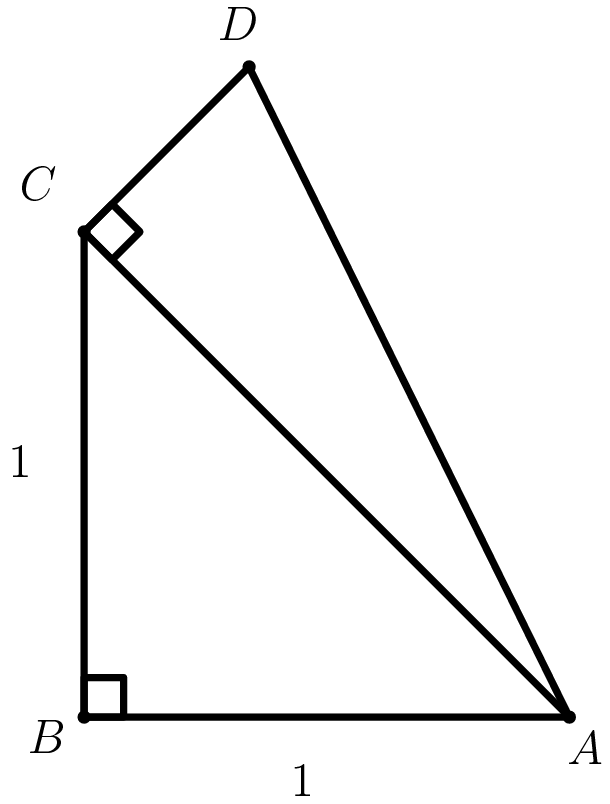
\includegraphics[width=0.3\linewidth]{2019AMC12B.png}    
    \end{figure}
\end{problem}

\begin{problem}
    (Denmark MO 2019) Pada gambar berikut, segitiga $BCD, CAE, $ dan $ABF$ merupakan segitiga sama sisi. Selain itu, segitiga $ABC$ adalah segitiga siku-siku dengan $\angle{A} = 90^{\circ}$. Jika $AD = 4$, panjang dari $EF$ adalah ...
    \begin{figure}[h]
        \centering
        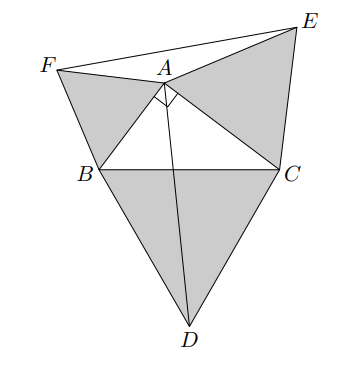
\includegraphics{DenmarkMO2019.png}
        \label{fig:my_label}
    \end{figure}
\end{problem}

\end{document}